\section{Modelización del sistema}
	\subsection{Actores}
		\paragraph\indent
		Un actor interactúa con el sistema, pudiendo ser estos un usuario u otro sistema. Los actores identificados son:
		\begin{itemize}
			\item Vendedores
			\item Fabricantes
			\item Administradores
		\end{itemize}
	\subsection{Diagrama de contexto}
	\begin{figure}[H]
		\centering
		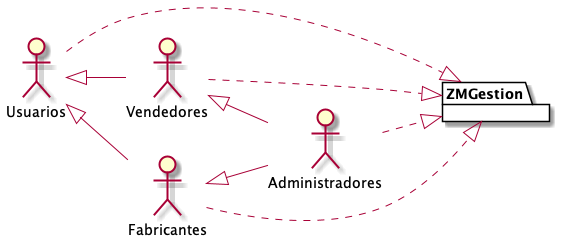
\includegraphics[width=\textwidth,height=0.40\textheight,keepaspectratio]{DiagramaContexto}
		\caption{Diagrama de contexto}
	\label{fig:DiagramaContexto}
    \end{figure}
    \subsection{Diagrama de subsistema}
	\begin{figure}[H]
		\centering
		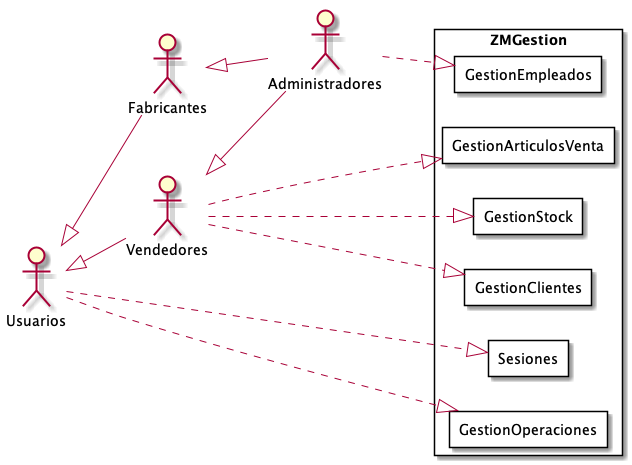
\includegraphics[width=\textwidth,height=0.40\textheight,keepaspectratio]{DiagramaSubsistema}
		\caption{Diagrama de subsistema}
	\label{fig:DiagramaSubsistema}
    \end{figure}
    
	\subsection{Diagrama de casos de uso}
	\begin{figure}[H]
		\centering
		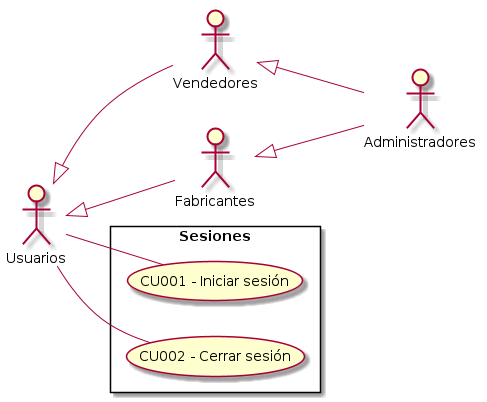
\includegraphics[width=\textwidth,height=0.90\textheight,keepaspectratio]{Sesiones}
		\caption{Diagrama de casos de uso para sesiones}
	\label{fig:Sesiones}
	\end{figure}
	\begin{figure}[H]
		\centering
		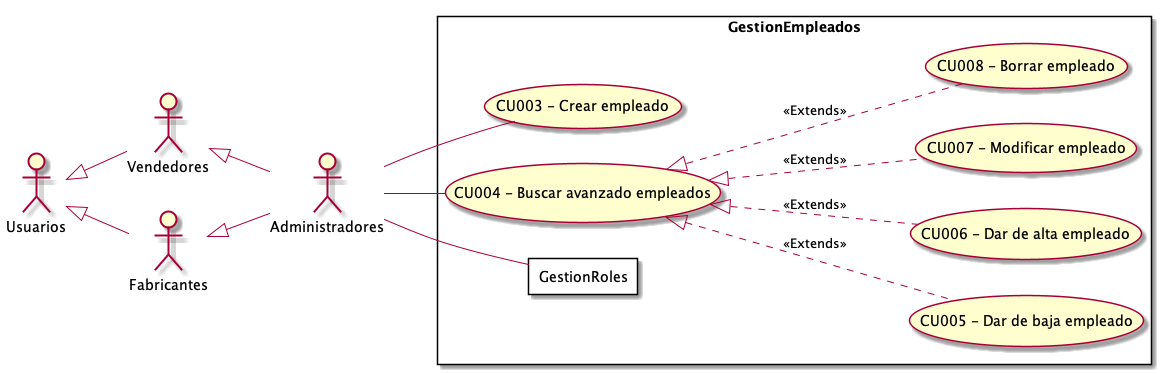
\includegraphics[width=\textwidth,height=0.90\textheight,keepaspectratio]{GestionEmpleados}
		\caption{Diagrama de casos de uso para la gestión de empleados}
	\label{fig:GestionEmpleados}
	\end{figure}
	\begin{figure}[H]
		\centering
		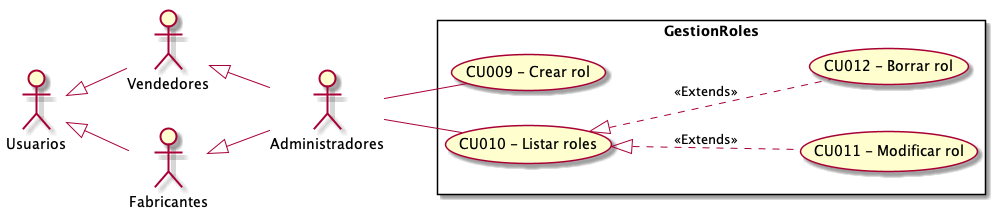
\includegraphics[width=\textwidth,height=0.90\textheight,keepaspectratio]{GestionRoles}
		\caption{Diagrama de casos de uso para la gestión de roles}
	\label{fig:GestionRoles}
    \end{figure}
    \begin{figure}[H]
		\centering
		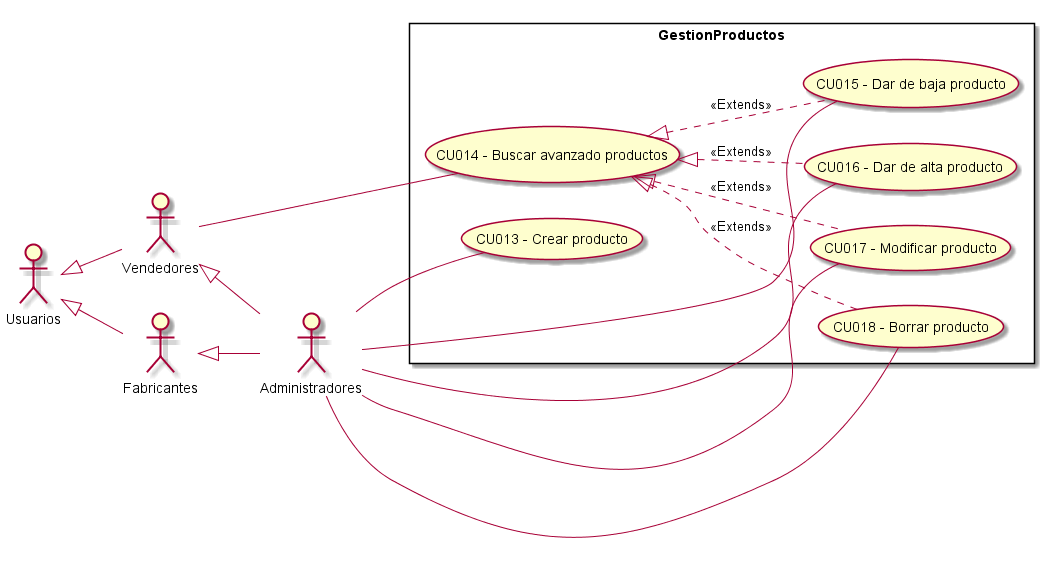
\includegraphics[width=\textwidth,height=0.90\textheight,keepaspectratio]{GestionProductos}
		\caption{Diagrama de casos de uso para la gestión de productos}
	\label{fig:GestionProductos}
    \end{figure}
    \begin{figure}[H]
		\centering
		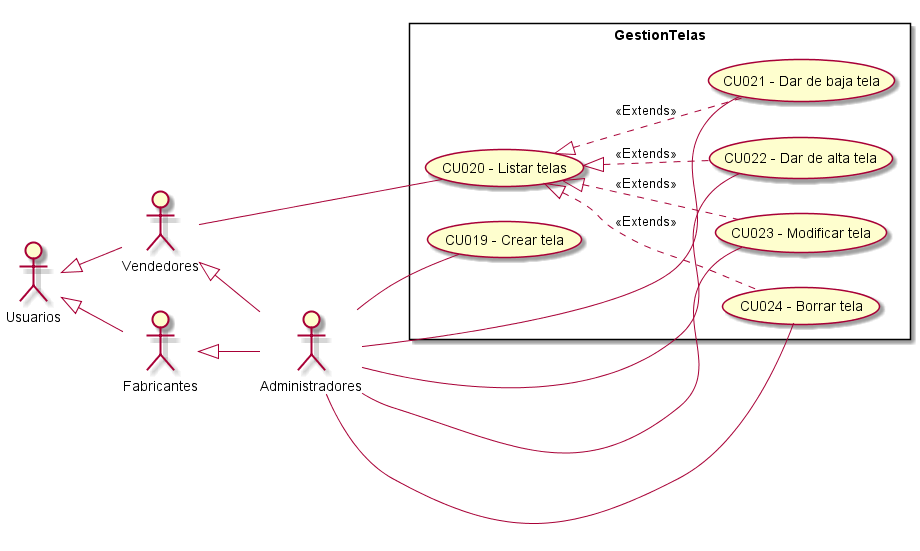
\includegraphics[width=\textwidth,height=0.90\textheight,keepaspectratio]{GestionTelas}
		\caption{Diagrama de casos de uso para la gestión de telas}
	\label{fig:GestionTelas}
    \end{figure}
    \begin{figure}[H]
		\centering
		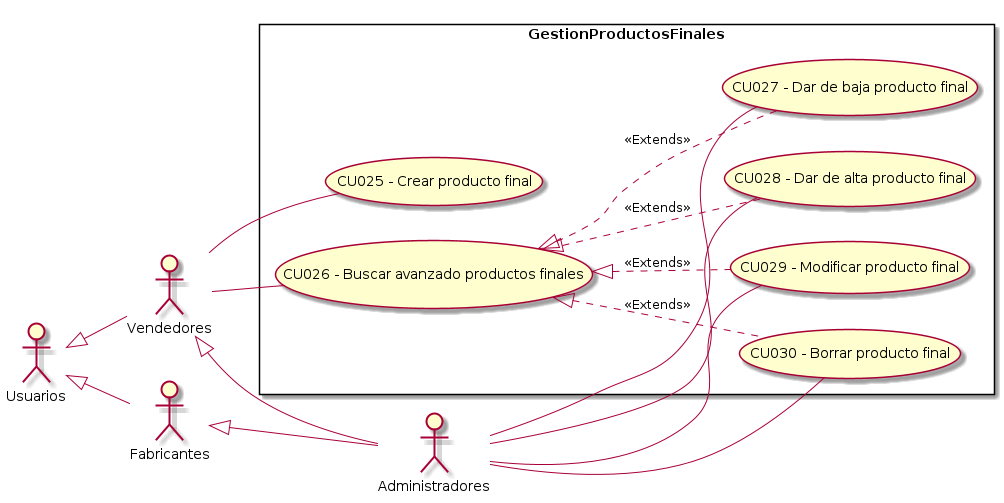
\includegraphics[width=\textwidth,height=0.90\textheight,keepaspectratio]{GestionProductosFinales}
		\caption{Diagrama de casos de uso para la gestión de productos finales}
	\label{fig:GestionProductosFinales}
    \end{figure}
    \begin{figure}[H]
		\centering
		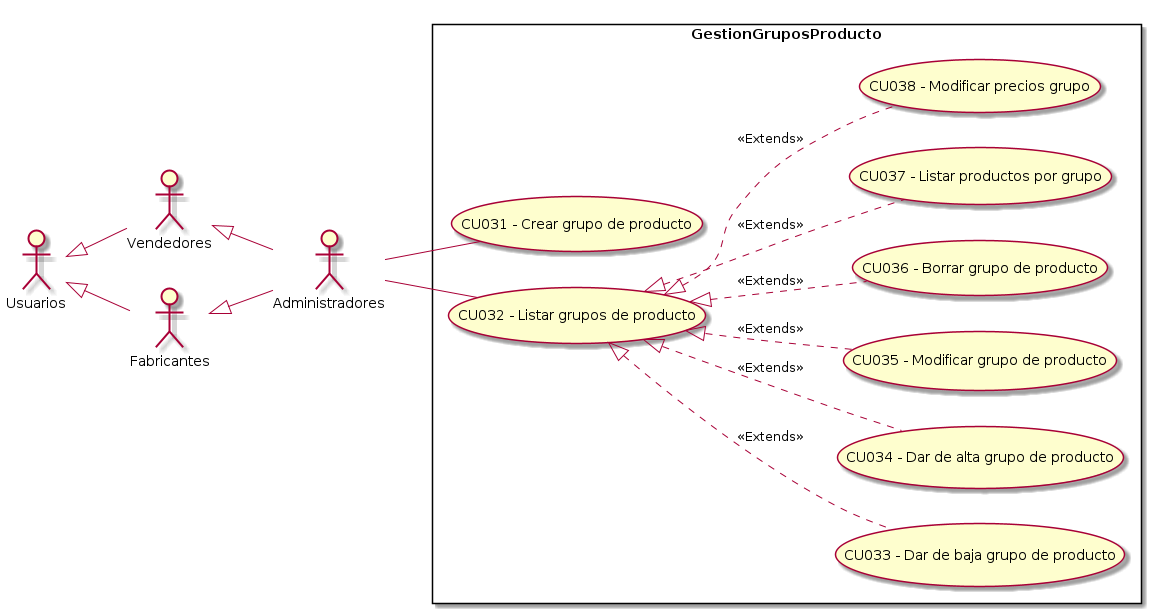
\includegraphics[width=\textwidth,height=0.90\textheight,keepaspectratio]{GestionGruposProducto}
		\caption{Diagrama de casos de uso para la gestión de grupos de producto}
	\label{fig:GestionGruposProducto}
    \end{figure}
    \begin{figure}[H]
		\centering
		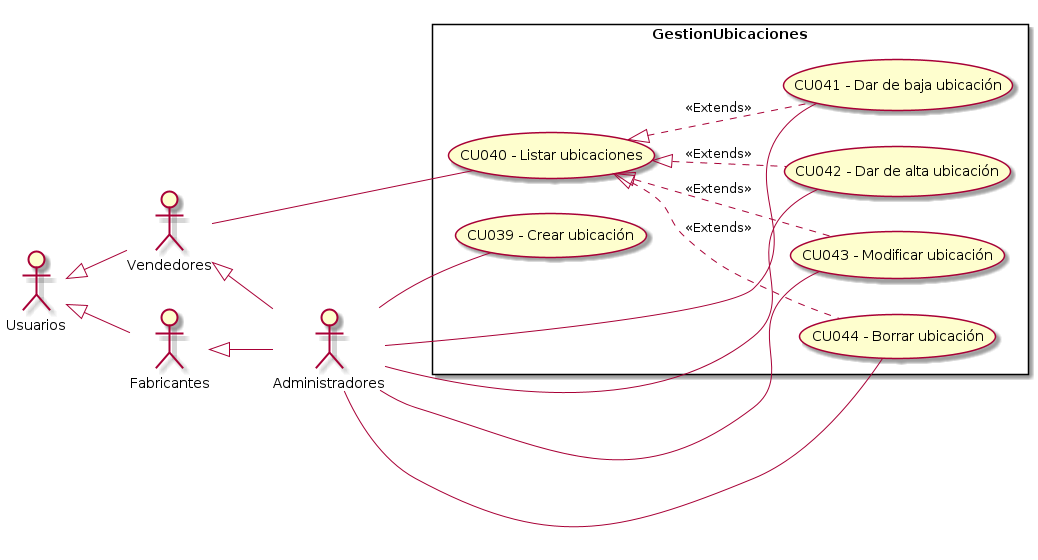
\includegraphics[width=\textwidth,height=0.90\textheight,keepaspectratio]{GestionUbicaciones}
		\caption{Diagrama de casos de uso para la gestión de ubicaciones}
	\label{fig:GestionUbicaciones}
    \end{figure}
    \begin{figure}[H]
		\centering
		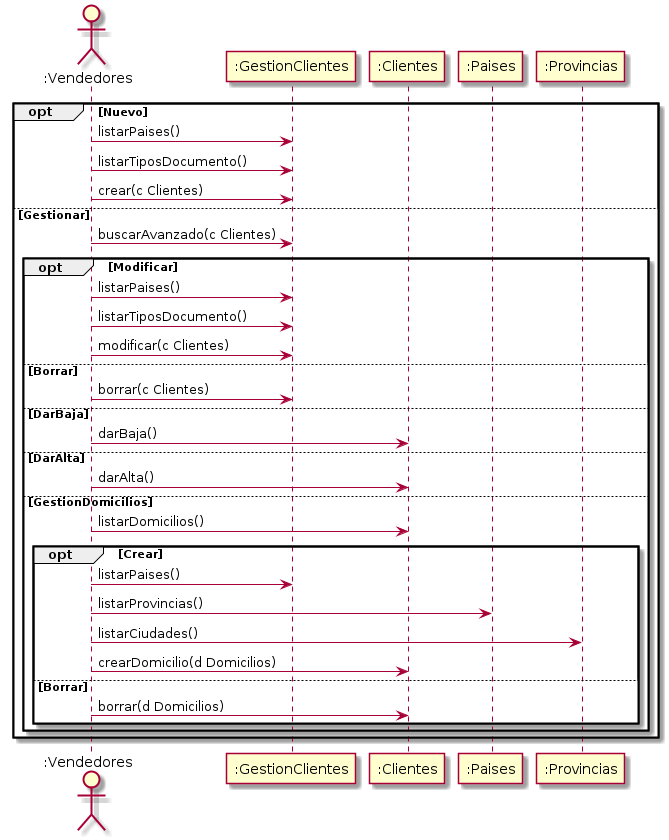
\includegraphics[width=\textwidth,height=0.90\textheight,keepaspectratio]{GestionClientes}
		\caption{Diagrama de casos de uso para la gestión de clientes}
	\label{fig:GestionClientes}
    \end{figure}
    \begin{figure}[H]
		\centering
		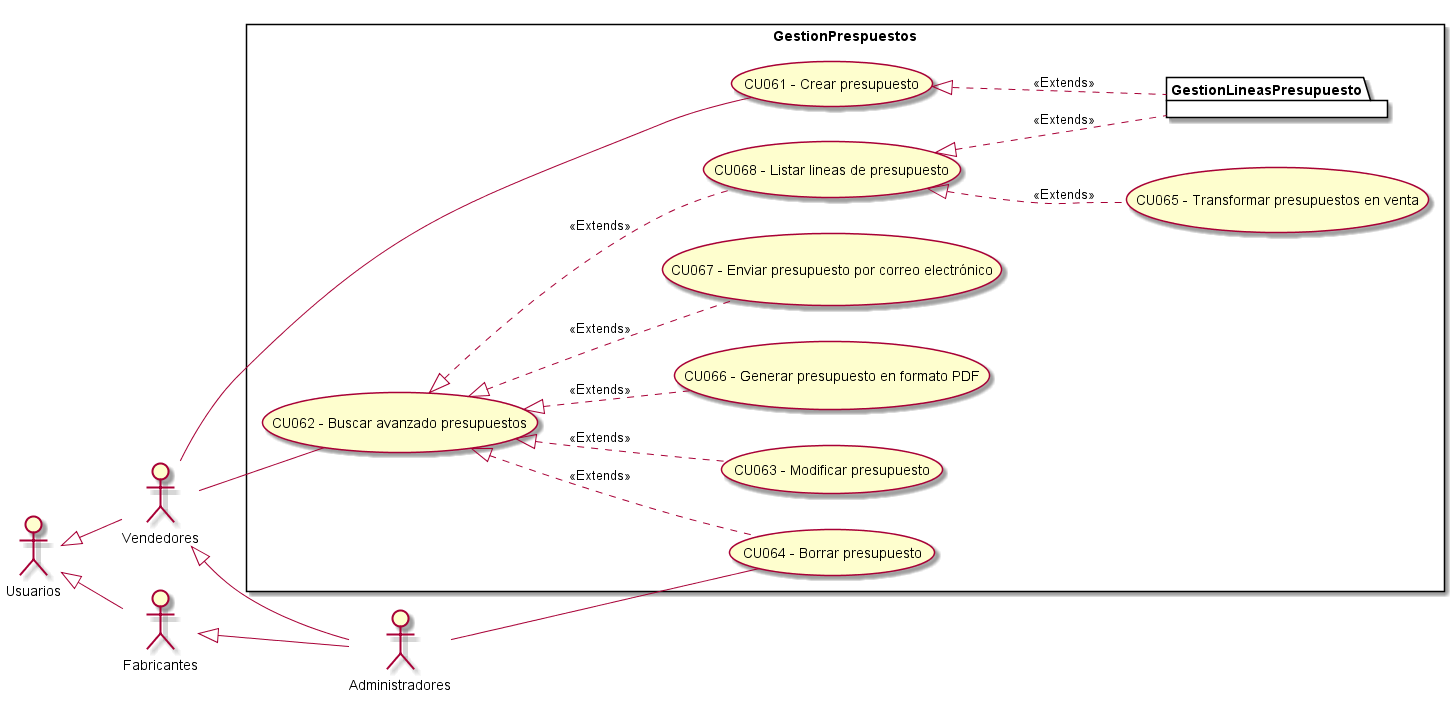
\includegraphics[width=\textwidth,height=0.90\textheight,keepaspectratio]{GestionPresupuestos}
		\caption{Diagrama de casos de uso para la gestión de presupuestos}
	\label{fig:GestionPresupuestos}
    \end{figure}
    \begin{figure}[H]
		\centering
		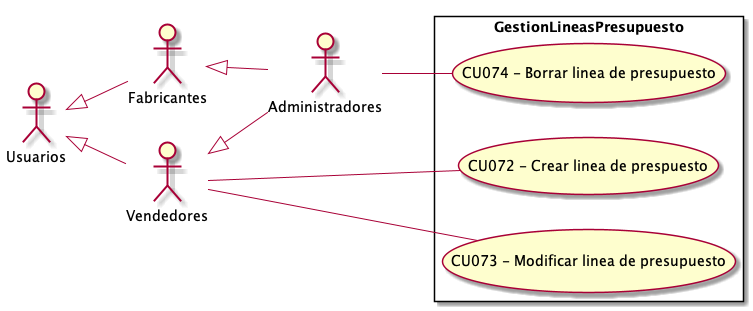
\includegraphics[width=\textwidth,height=0.90\textheight,keepaspectratio]{GestionLineasPresupuesto}
		\caption{Diagrama de casos de uso para la gestión de líneas de presupuesto}
	\label{fig:GestionLineasPresupuesto}
    \end{figure}
    \begin{figure}[H]
		\centering
		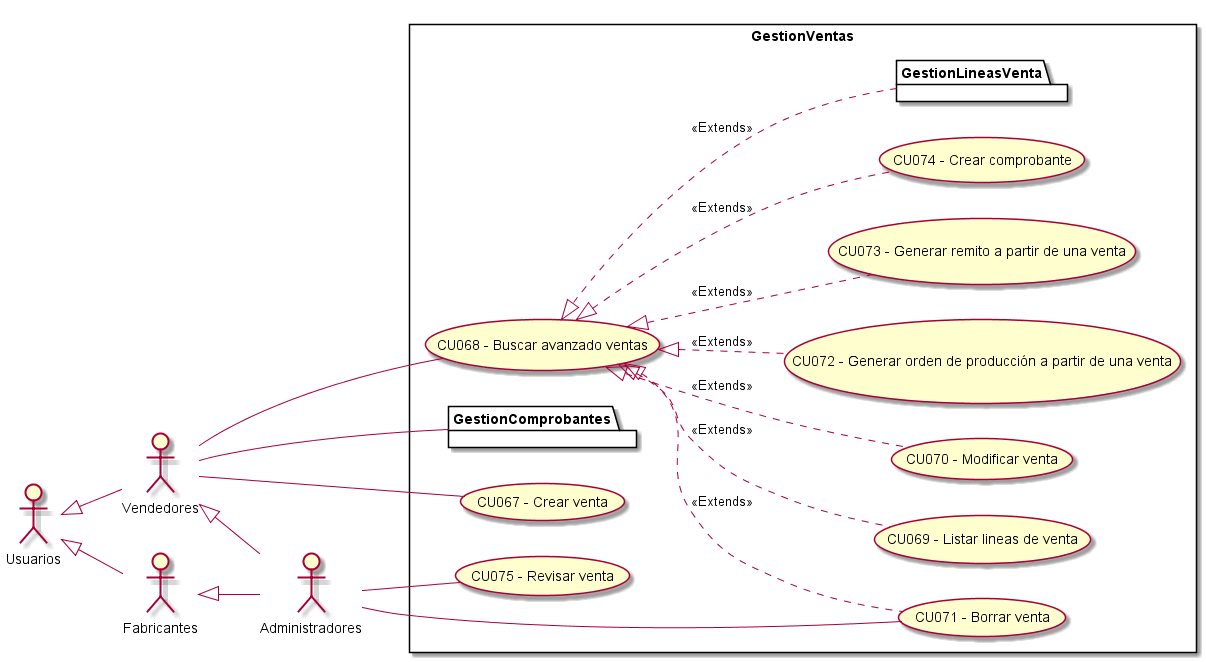
\includegraphics[width=\textwidth,height=0.90\textheight,keepaspectratio]{GestionVentas}
		\caption{Diagrama de casos de uso para la gestión de ventas}
	\label{fig:GestionVentas}
    \end{figure}
    \begin{figure}[H]
		\centering
		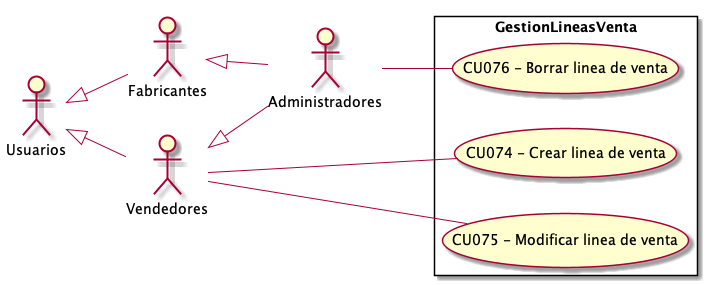
\includegraphics[width=\textwidth,height=0.90\textheight,keepaspectratio]{GestionLineasVenta}
		\caption{Diagrama de casos de uso para la gestión de líneas de venta}
	\label{fig:GestionLineasVenta}
    \end{figure}
    \begin{figure}[H]
		\centering
		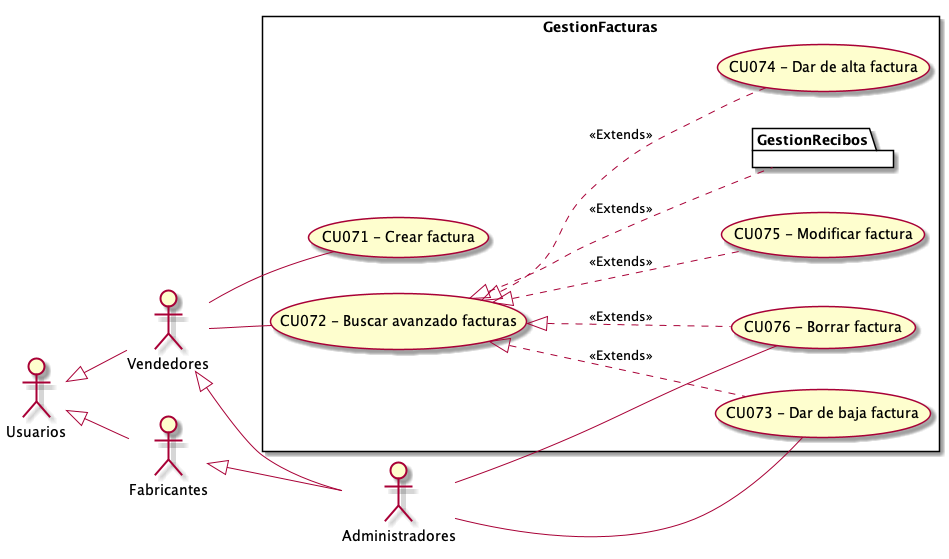
\includegraphics[width=\textwidth,height=0.90\textheight,keepaspectratio]{GestionFacturas}
		\caption{Diagrama de casos de uso para la gestión de facturas}
	\label{fig:GestionFacturas}
    \end{figure}
    \begin{figure}[H]
		\centering
		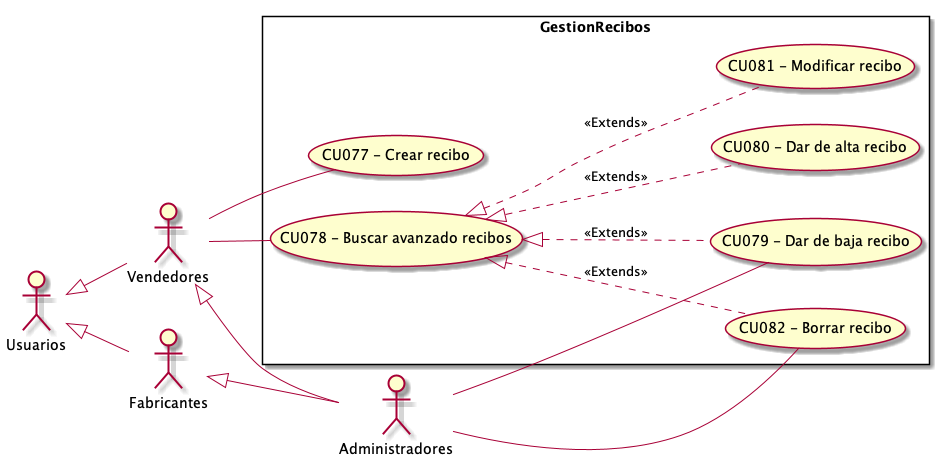
\includegraphics[width=\textwidth,height=0.90\textheight,keepaspectratio]{GestionRecibos}
		\caption{Diagrama de casos de uso para la gestión de recibos}
	\label{fig:GestionRecibos}
    \end{figure}
    \begin{figure}[H]
		\centering
		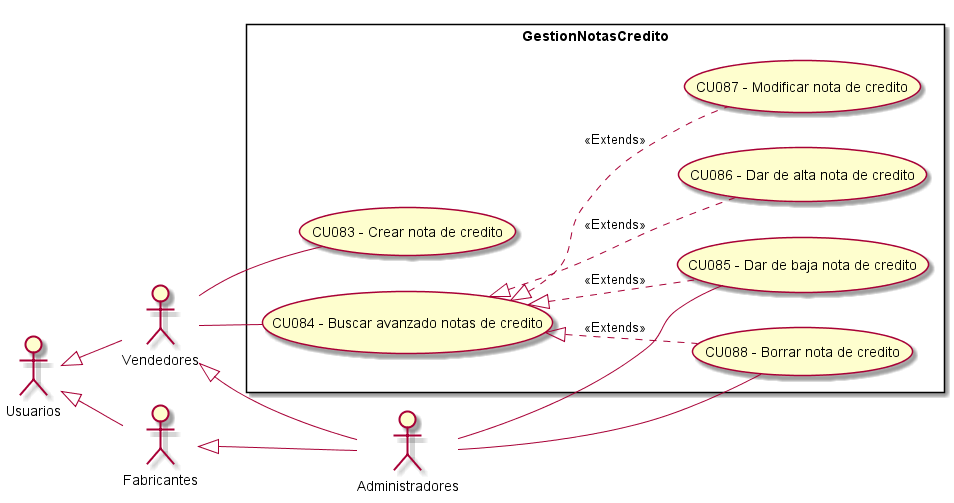
\includegraphics[width=\textwidth,height=0.90\textheight,keepaspectratio]{GestionNotasCredito}
		\caption{Diagrama de casos de uso para la gestión de notas de crédito}
	\label{fig:GestionNotasCredito}
    \end{figure}
    \begin{figure}[H]
		\centering
		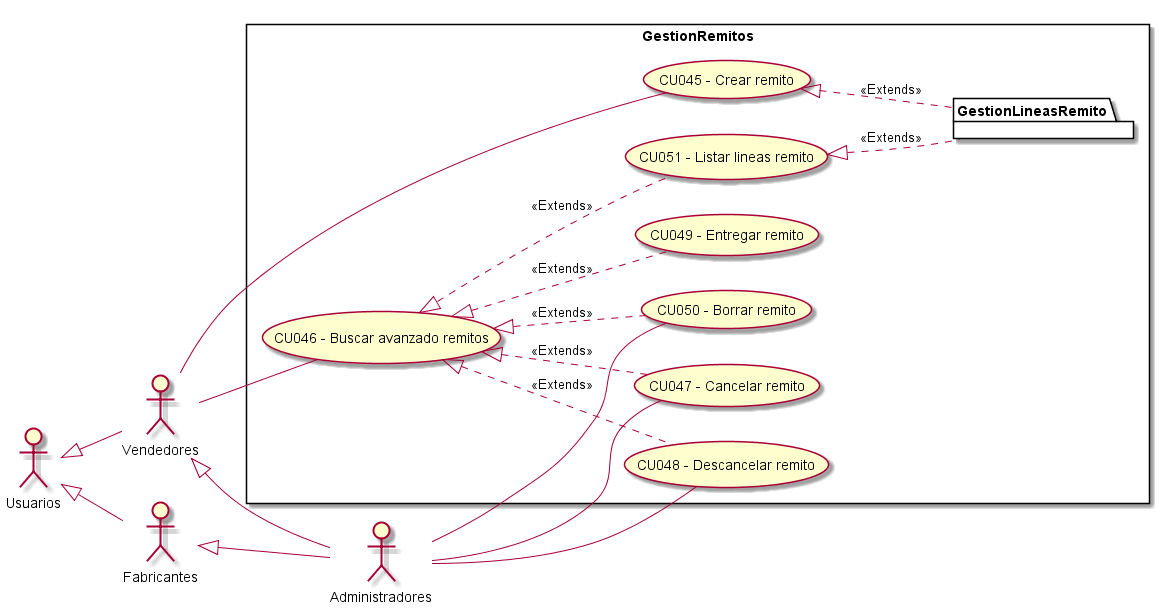
\includegraphics[width=\textwidth,height=0.90\textheight,keepaspectratio]{GestionRemitos}
		\caption{Diagrama de casos de uso para la gestión de remitos}
	\label{fig:GestionRemitos}
    \end{figure}
    \begin{figure}[H]
		\centering
		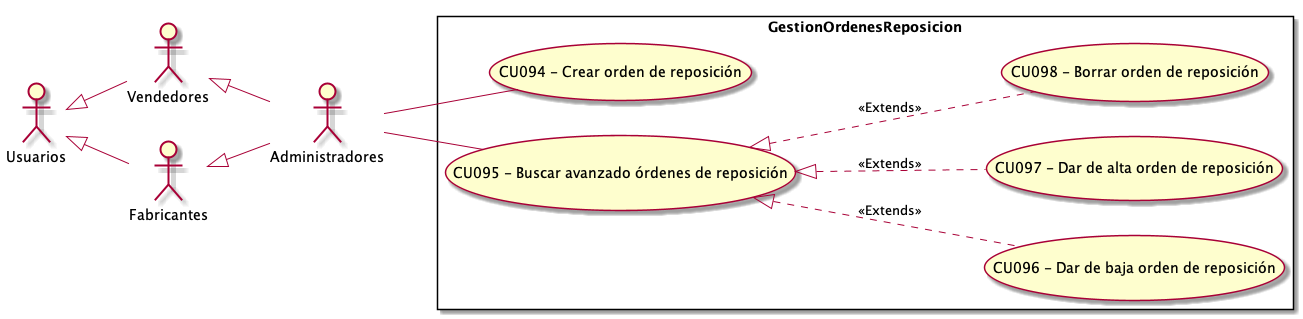
\includegraphics[width=\textwidth,height=0.90\textheight,keepaspectratio]{GestionOrdenesReposicion}
		\caption{Diagrama de casos de uso para la gestión de órdenes de reposición}
	\label{fig:GestionOrdenesReposicion}
    \end{figure}
    \begin{figure}[H]
		\centering
		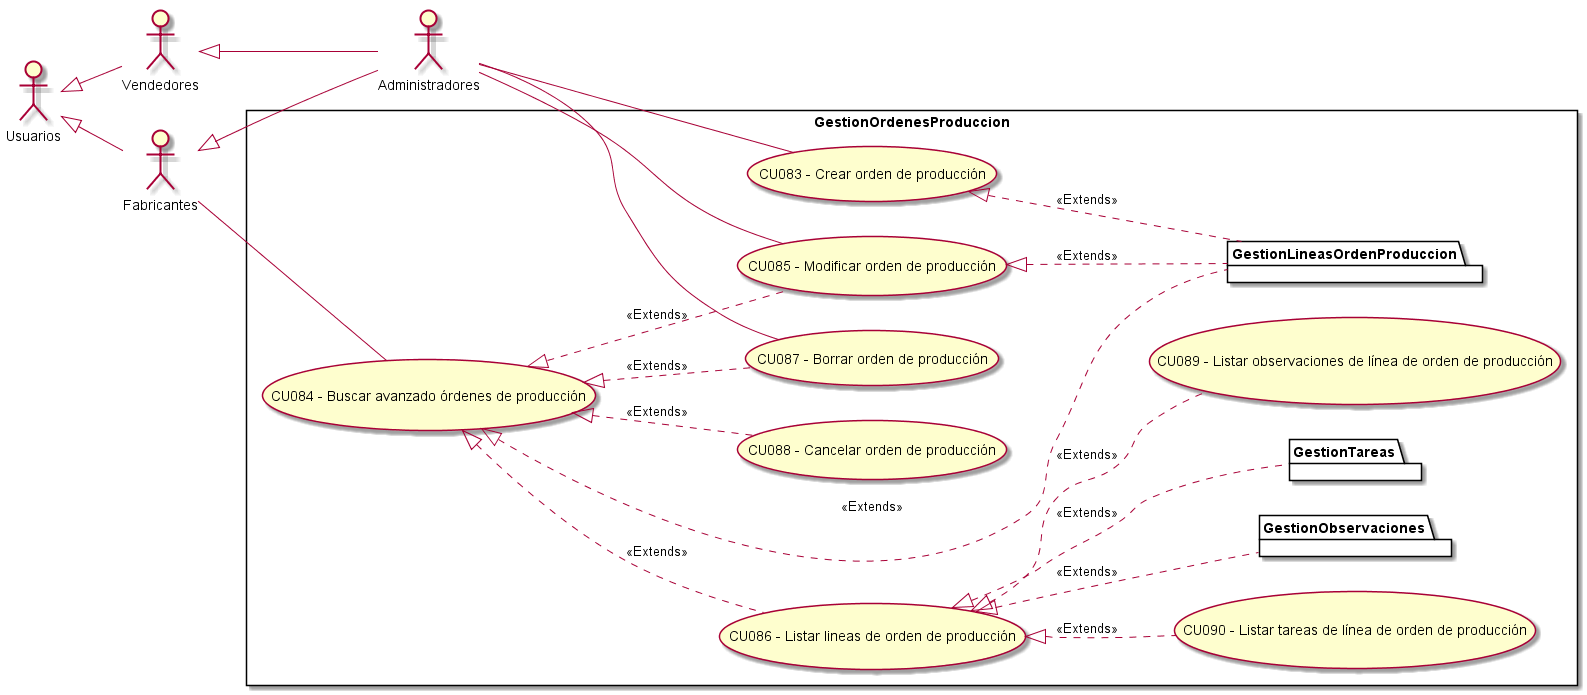
\includegraphics[width=\textwidth,height=0.90\textheight,keepaspectratio]{GestionOrdenesProduccion}
		\caption{Diagrama de casos de uso para la gestión de órdenes de producción}
	\label{fig:GestionOrdenesProduccion}
    \end{figure}
    \begin{figure}[H]
		\centering
		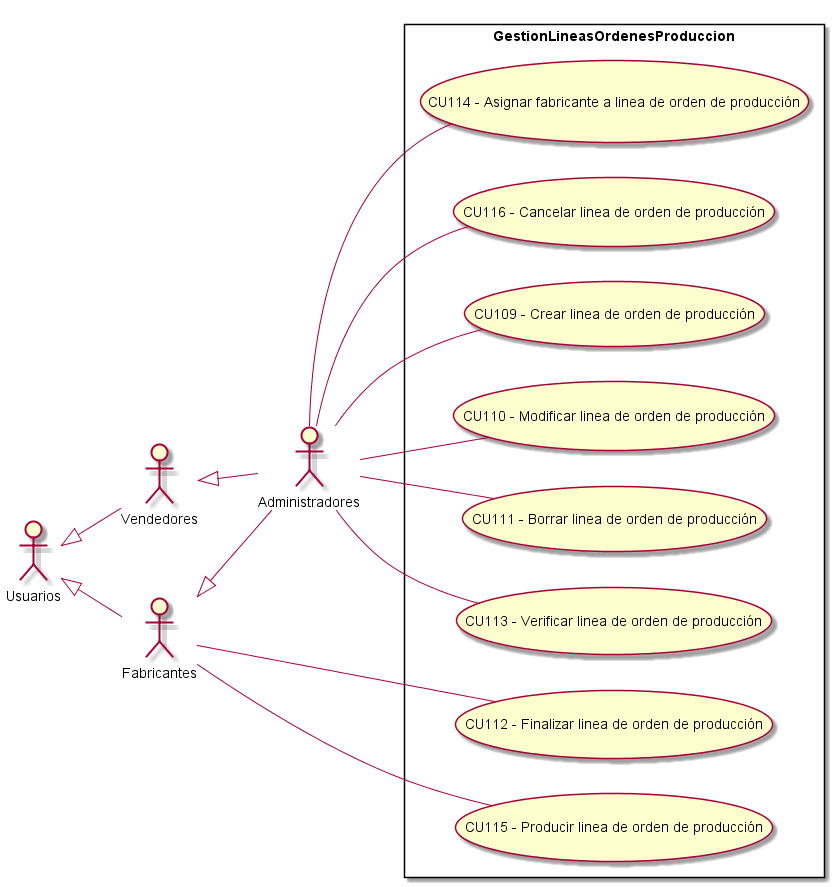
\includegraphics[width=\textwidth,height=0.90\textheight,keepaspectratio]{GestionLineasOrdenesProduccion}
		\caption{Diagrama de casos de uso para la gestión de líneas de órdenes de producción}
	\label{fig:GestionLineasOrdenesProduccion}
    \end{figure}
    \begin{figure}[H]
		\centering
		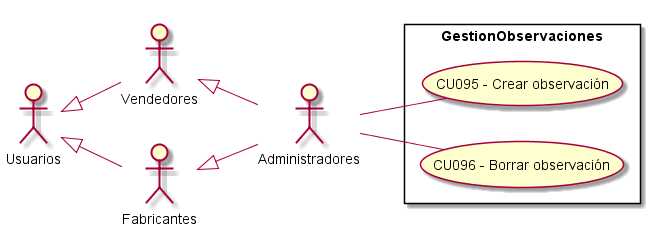
\includegraphics[width=\textwidth,height=0.90\textheight,keepaspectratio]{GestionObservaciones}
		\caption{Diagrama de casos de uso para la gestión de observaciones}
	\label{fig:GestionObservaciones}
    \end{figure}
    